\documentclass[12pt]{article}

\usepackage[top=1in, bottom=1in, left=1.2in, right=1in]{geometry}
\pagestyle{plain}
\linespread{1.5}

\usepackage[utf8]{inputenc}
\usepackage{float}
\usepackage[spanish]{babel}
\usepackage{graphicx}
\usepackage{listings}
\usepackage{color}
\usepackage{datetime}
\usepackage{csquotes}
\usepackage[table,xcdraw]{xcolor}
\usepackage{pdfpages}
\newdate{date}{30}{04}{2019}

\begin{document}

\definecolor{codegreen}{rgb}{0,0.6,0}
\definecolor{codegray}{rgb}{0.5,0.5,0.5}
\definecolor{codepurple}{rgb}{0.58,0,0.82}
\definecolor{backcolour}{rgb}{0.95,0.95,0.92}
 
\lstdefinestyle{mystyle}{
    backgroundcolor=\color{backcolour},   
    commentstyle=\color{codegreen},
    keywordstyle=\color{magenta},
    numberstyle=\tiny\color{codegray},
    stringstyle=\color{codepurple},
    basicstyle=\footnotesize,
    breakatwhitespace=false,         
    breaklines=true,                 
    captionpos=b,                    
    keepspaces=true,                 
    numbers=left,                    
    numbersep=5pt,                  
    showspaces=false,                
    showstringspaces=false,
    showtabs=false,                  
    tabsize=2
}
 
\lstset{style=mystyle}


\begin{titlepage}
\begin{figure}[t]
    \centering
\includegraphics[width=0.3\textwidth]{logouanl}
\end{figure}
\begin{center}
    \textsc{ \LARGE{Universidad Autonoma de Nuevo León \\}}
	\textsc{ \LARGE{Facultad de Ingenieria Mecánica y Eléctrica\\ }}
	\textnormal{ \LARGE{Optimización de flujo en redes\\}}
	\vspace{30mm}
	\fontsize{10mm}{7mm}\selectfont 
    \textup{Portafolio de Tareas}\\
\end{center}

\vspace{25mm}

\begin{minipage}[t]{0.47\textwidth}
	\textnormal{\large{\bf Alumno:\\}}
	{\large Jesús Angel Patlán Castillo}
\end{minipage}\hfill\begin{minipage}[t]{0.47\textwidth}\raggedleft
	\textnormal{\large{\bf Matricula:\\}}
	{\large 1595261}
\end{minipage}

\vspace{20mm}

\centering{\large{Enero - Junio 2019 \\ Fecha - 04/06/19 }}

\end{titlepage}

\pagebreak
\section{Introducción}
Este documento recopila las tareas de la materia Optimización de flujo en redes realizadas durante el periodo Enero-Junio 2019. Cada una de las tareas esta calificadas por la Dra. Satu Elisa Schaeffer, con anotaciones de aspectos a mejorar; los cuales fueron considerados para ser corregidos en esta recopilación.
Se muestra cada tarea con una lista con los puntos corregidos, posteriormente se muestra la tarea con las anotaciones y finalmente, si se considera necesario, la tarea con las nuevas correcciones.
Al final del documento, se incluye la conclusión de aprendizaje del curso.
Estas tareas se encuentran dentro de mi repositorio personal \cite{JAPC}.
\pagebreak
\section{Tarea 1}
Para esta tarea:
\begin{itemize}
    \item Se realizaron pequeñas correcciones al documento de diseño y errores ortográficos.
\end{itemize}
Dado que las correcciones no muestran un cambio significativo al documento, se decide no mostrar la nueva versión.
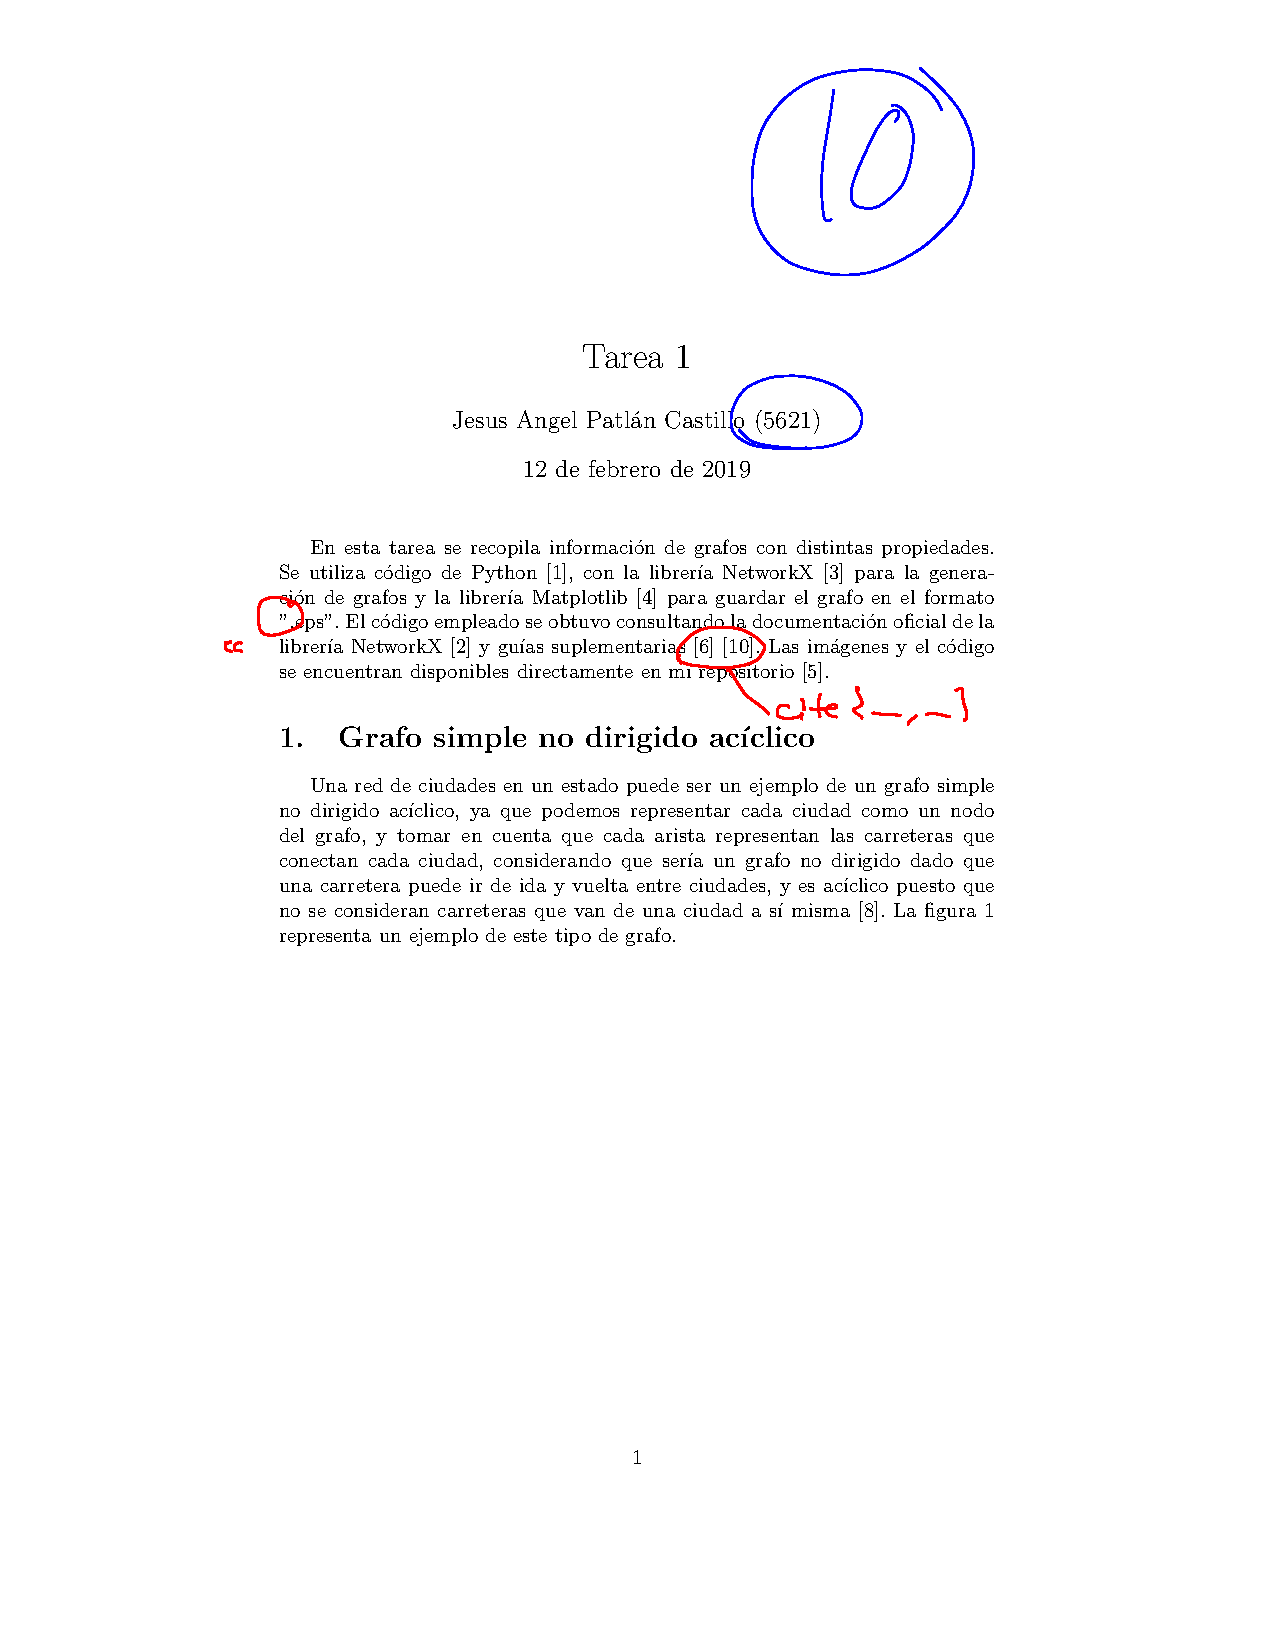
\includepdf[page=-]{5261-1}

\section{Tarea 2}
Para esta tarea:
\begin{itemize}
    \item Se realizaron pequeñas correcciones al documento de diseño y errores ortográficos.
    \item Se tradujeron las palabras que venían en inglés a español para mantener el mismo idioma en el documento.
    \item Se hizo un reacomodo en las referencias del documento.
\end{itemize}
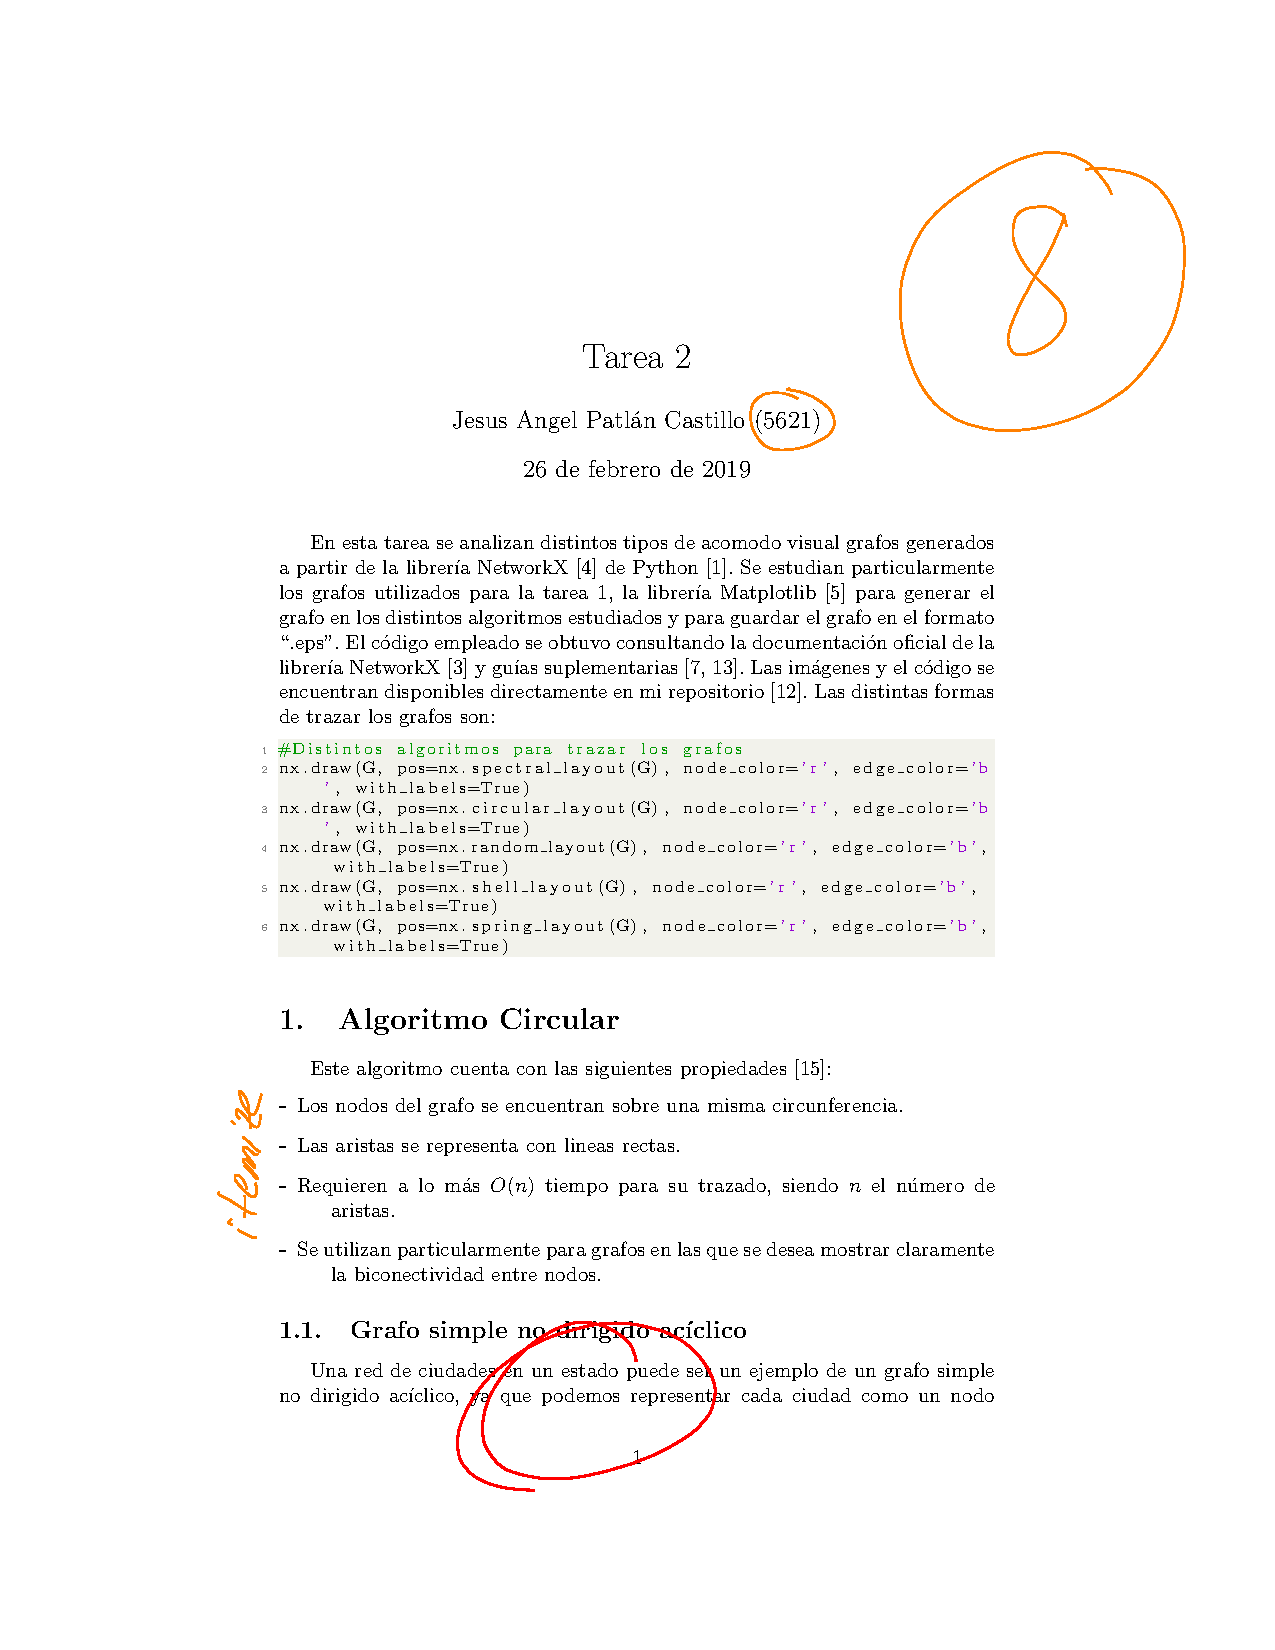
\includepdf[page=-]{5261-2}
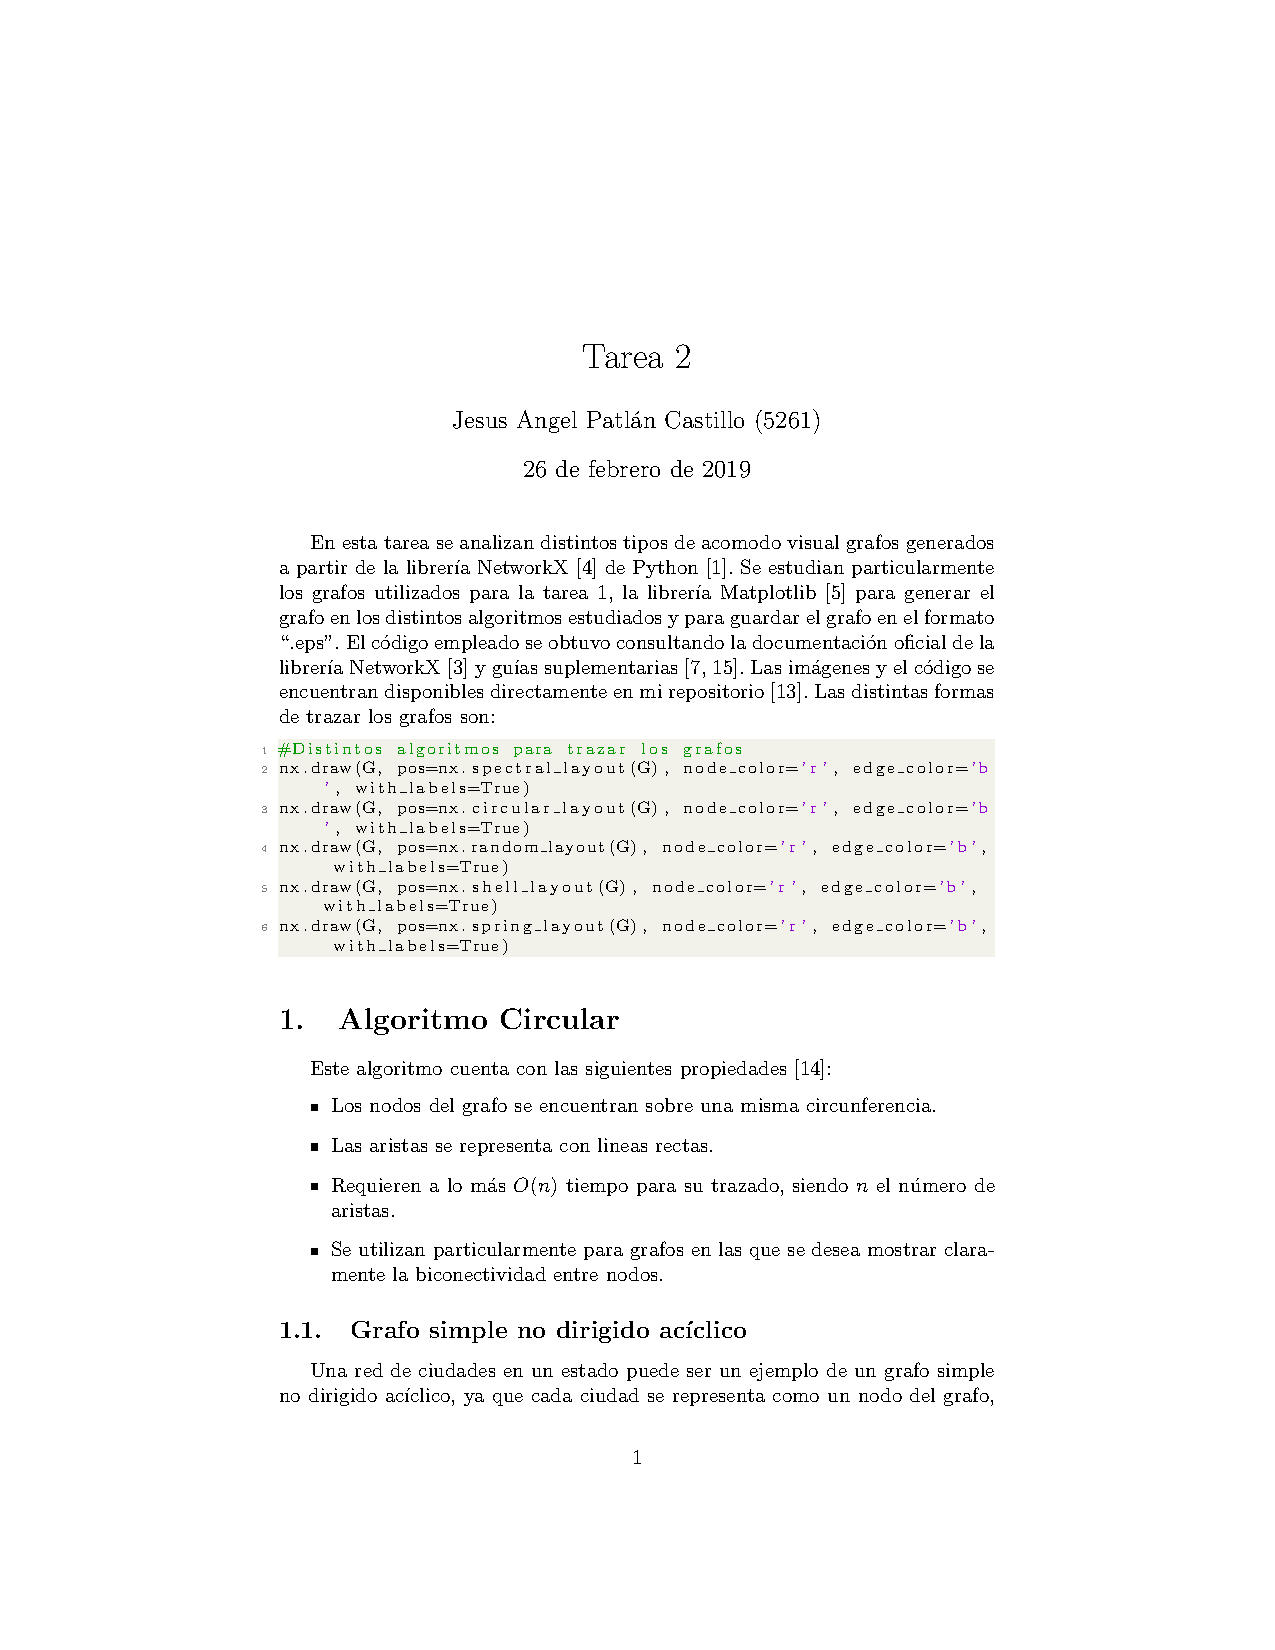
\includepdf[page=-]{5261-2-R}

\section{Tarea 3}
Para esta tarea:
\begin{itemize}
    \item Se realizaron pequeñas correcciones al documento de diseño y errores ortográficos.
\end{itemize}
Dado que las correcciones no muestran un cambio significativo al documento, se decide no mostrar la nueva versión.
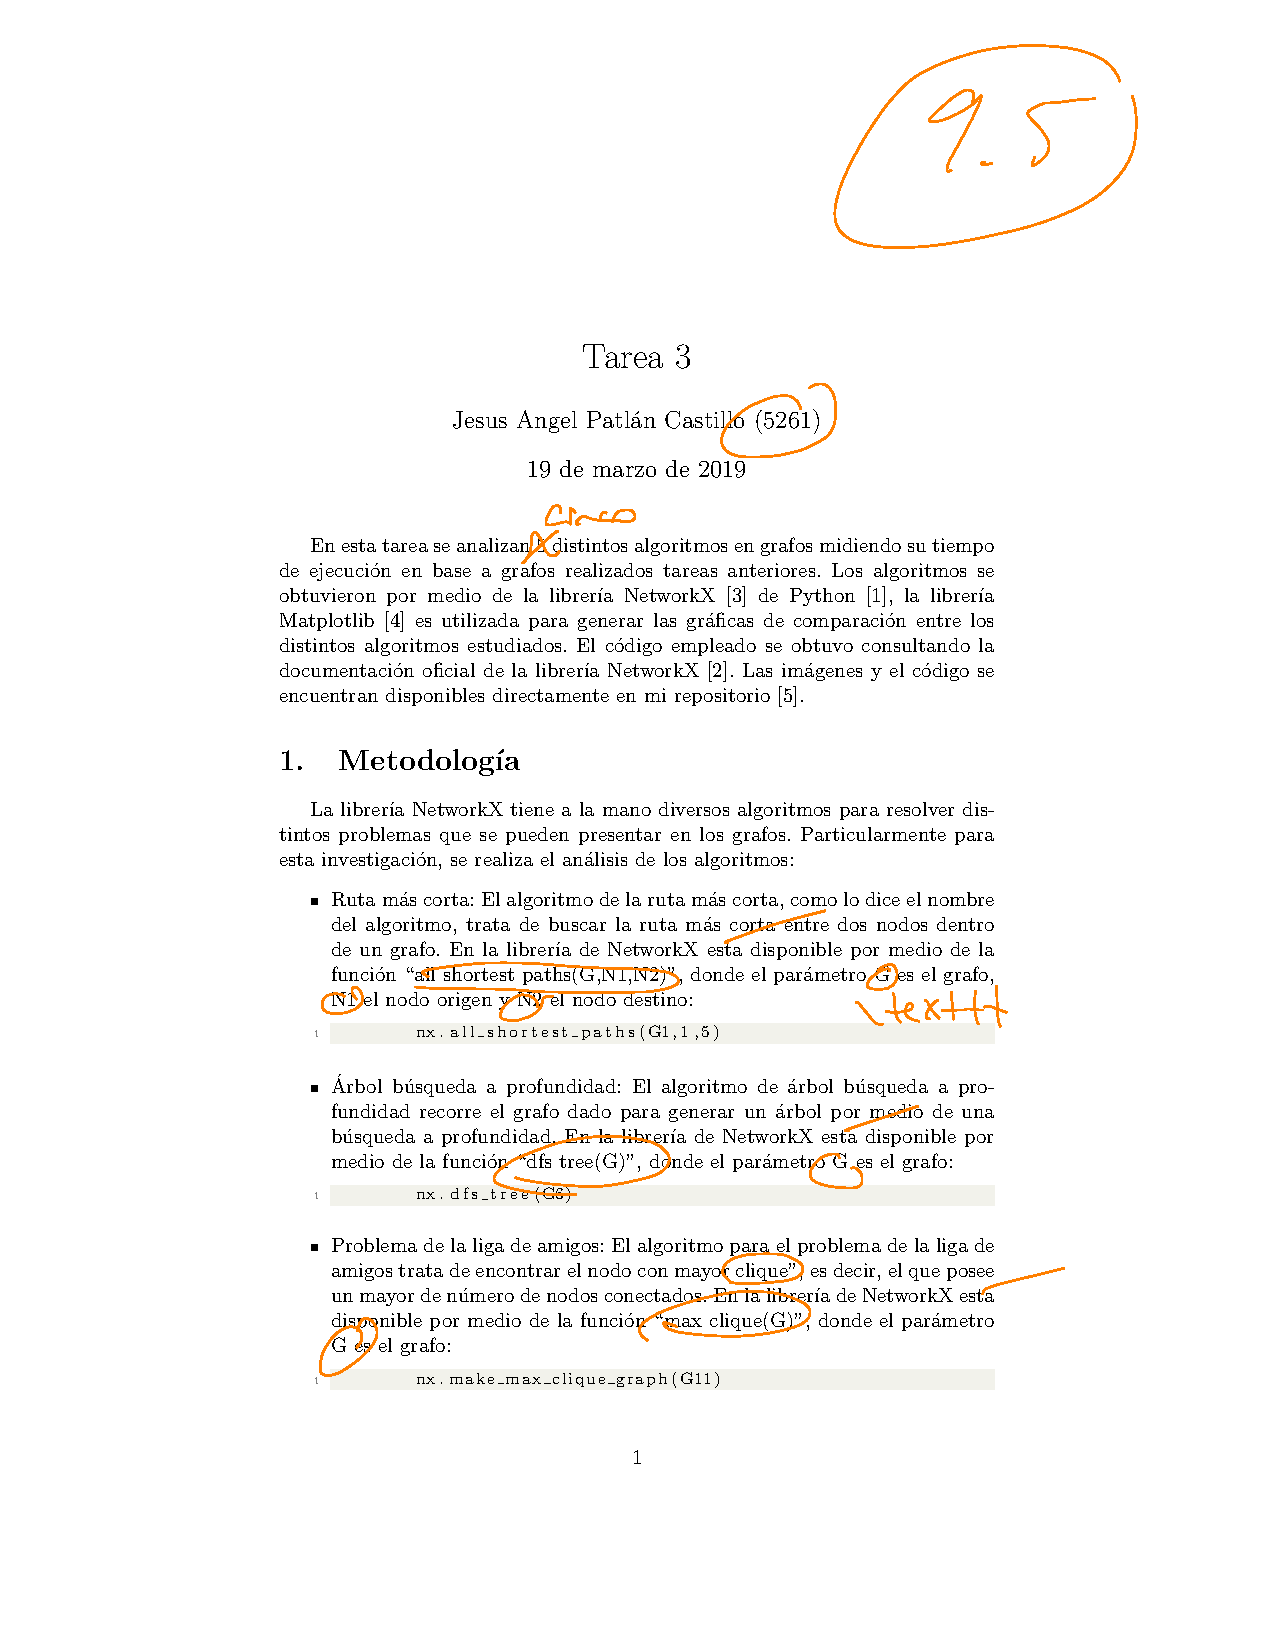
\includepdf[page=-]{5261-3}

\section{Tarea 4}
Para esta tarea:
\begin{itemize}
    \item Se realizaron pequeñas correcciones al documento de diseño y errores ortográficos.
    \item Se arreglo el código presente en el documento.
    \item Se ajustaron los valores P mostrados en la tabla ANOVA, mostrando solo hasta 2 decimales.
    \item Se agregaron gráficas que apoyan los resultados y las conclusiones.
\end{itemize}
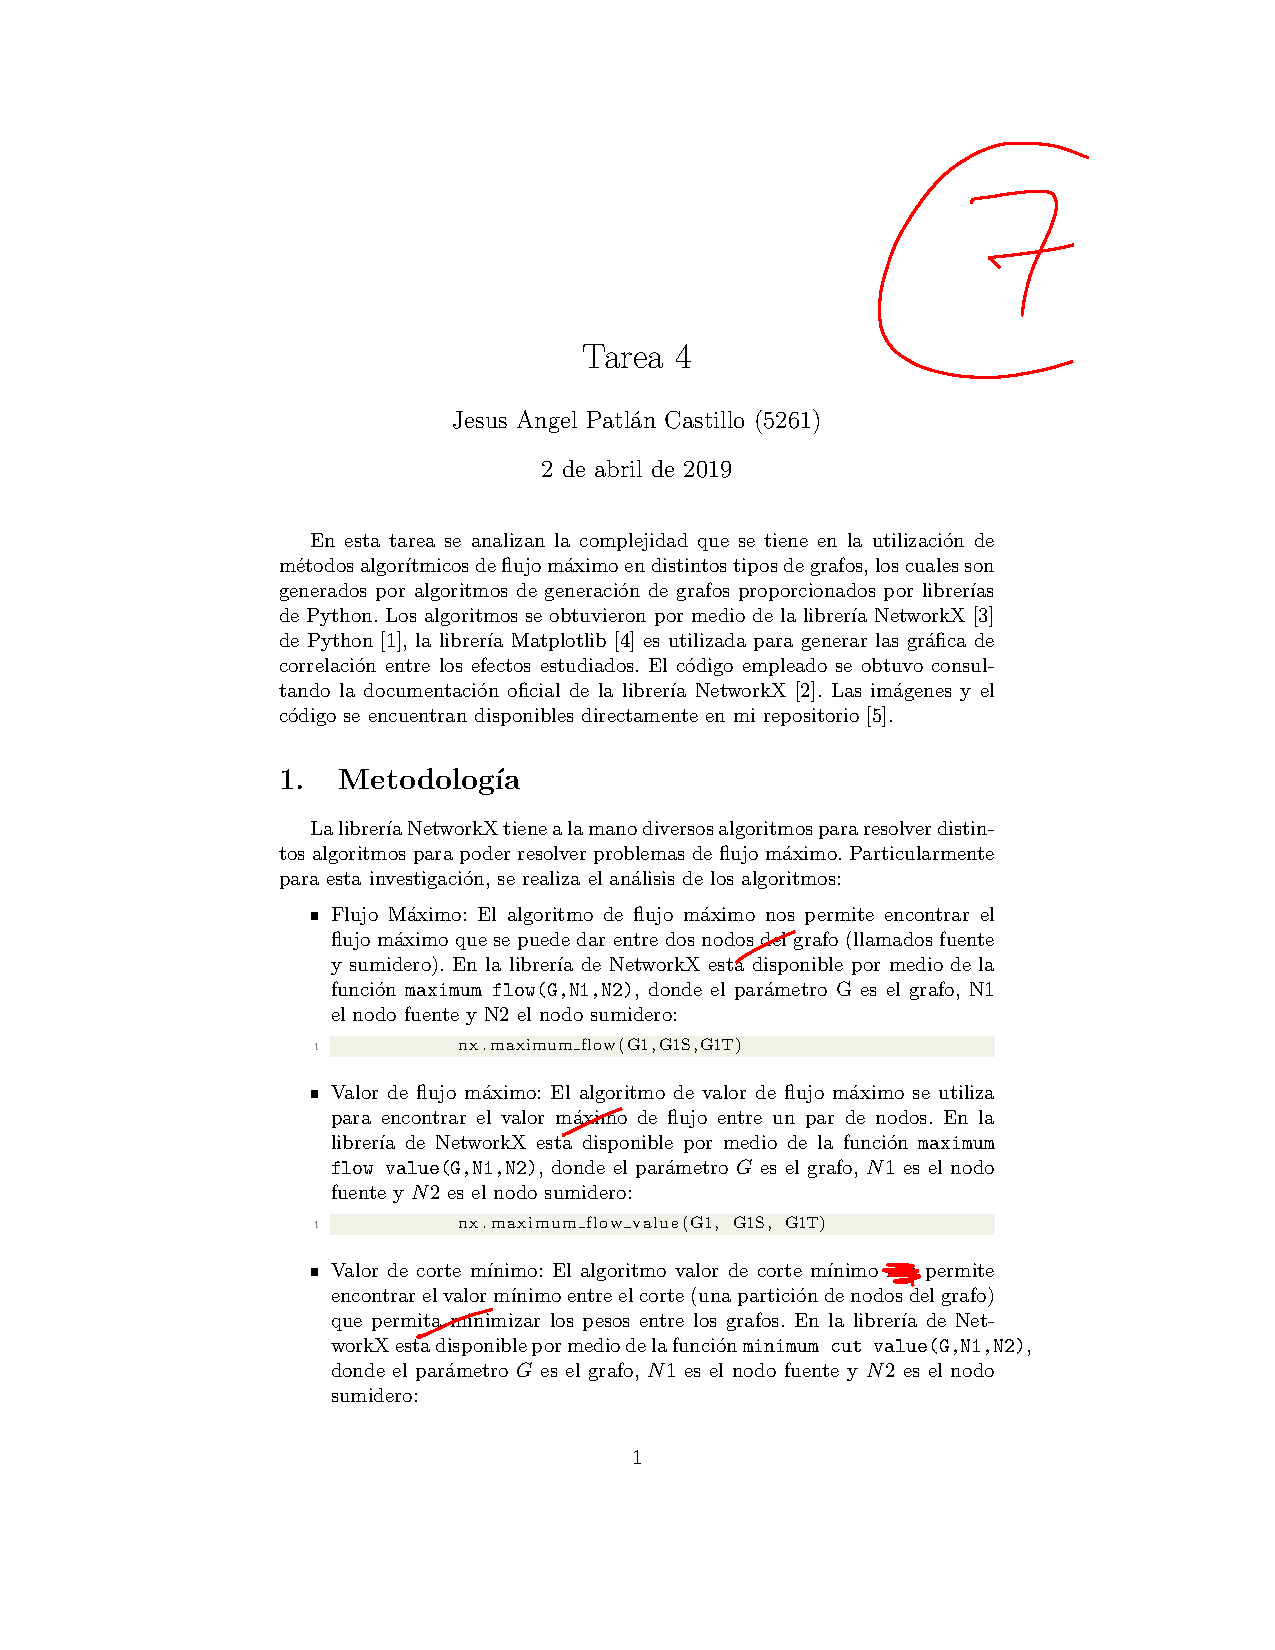
\includepdf[page=-]{5261-4}
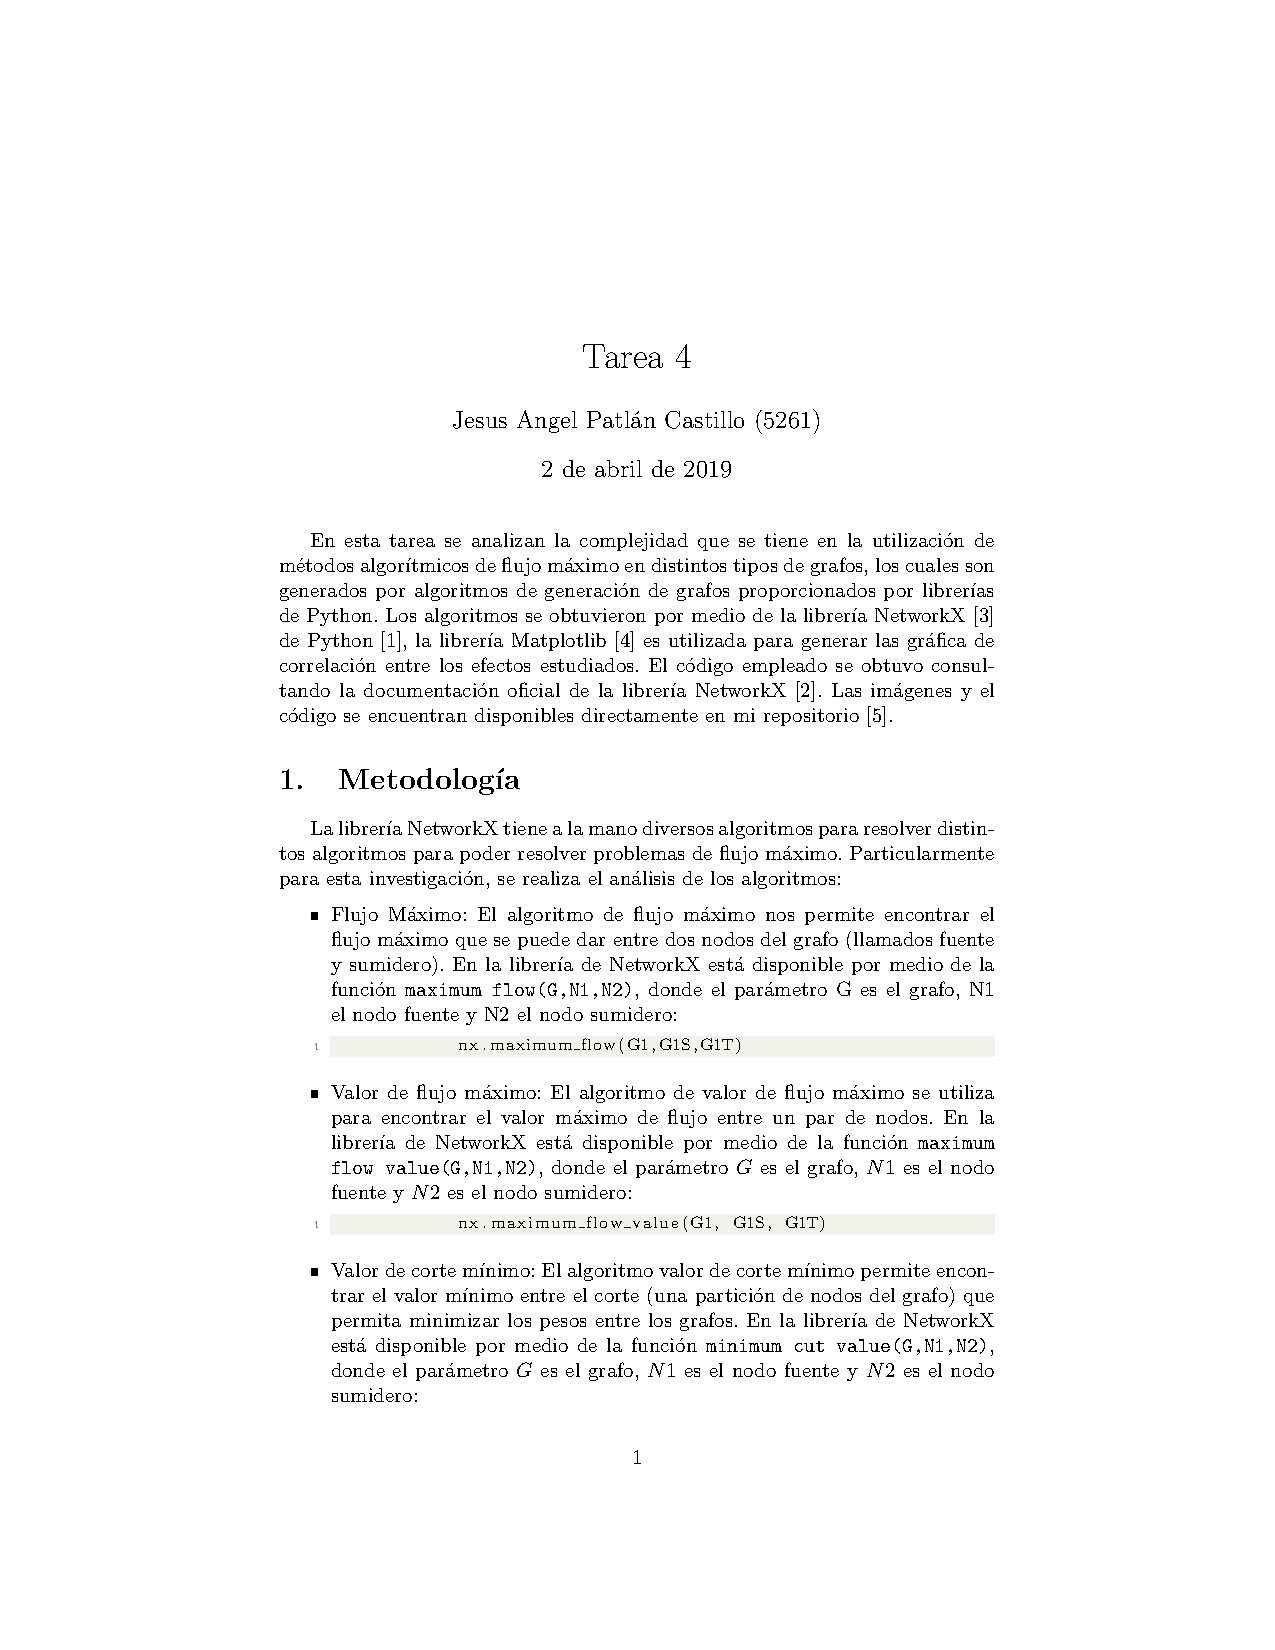
\includepdf[page=-]{5261-4-R}

\section{Tarea 5}
Para esta tarea:
\begin{itemize}
    \item Se realizaron pequeñas correcciones al documento de diseño y errores ortográficos.
    \item Se arreglo cambio el formato de la tabla a Latex.
    \item Se agregaron gráficas que apoyan los resultados y las conclusiones.
\end{itemize}
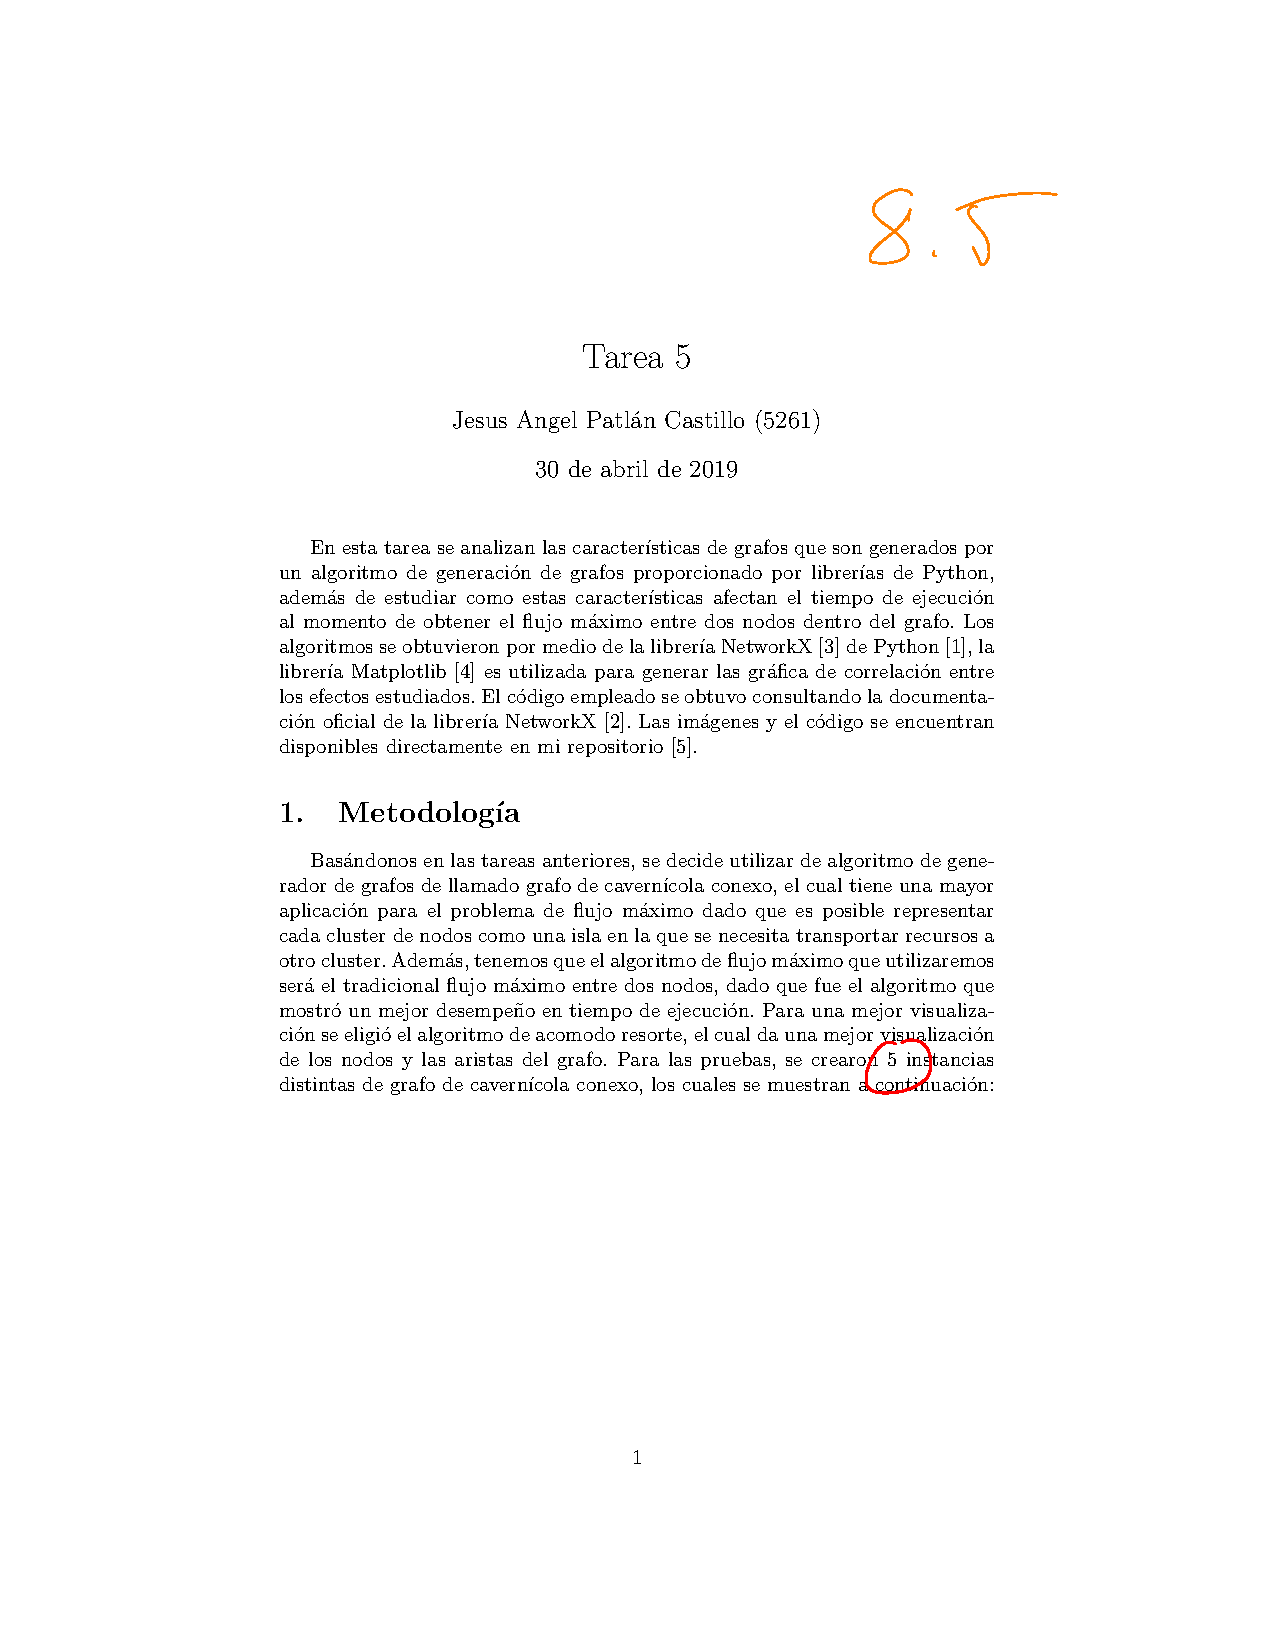
\includepdf[page=-]{5261-5}
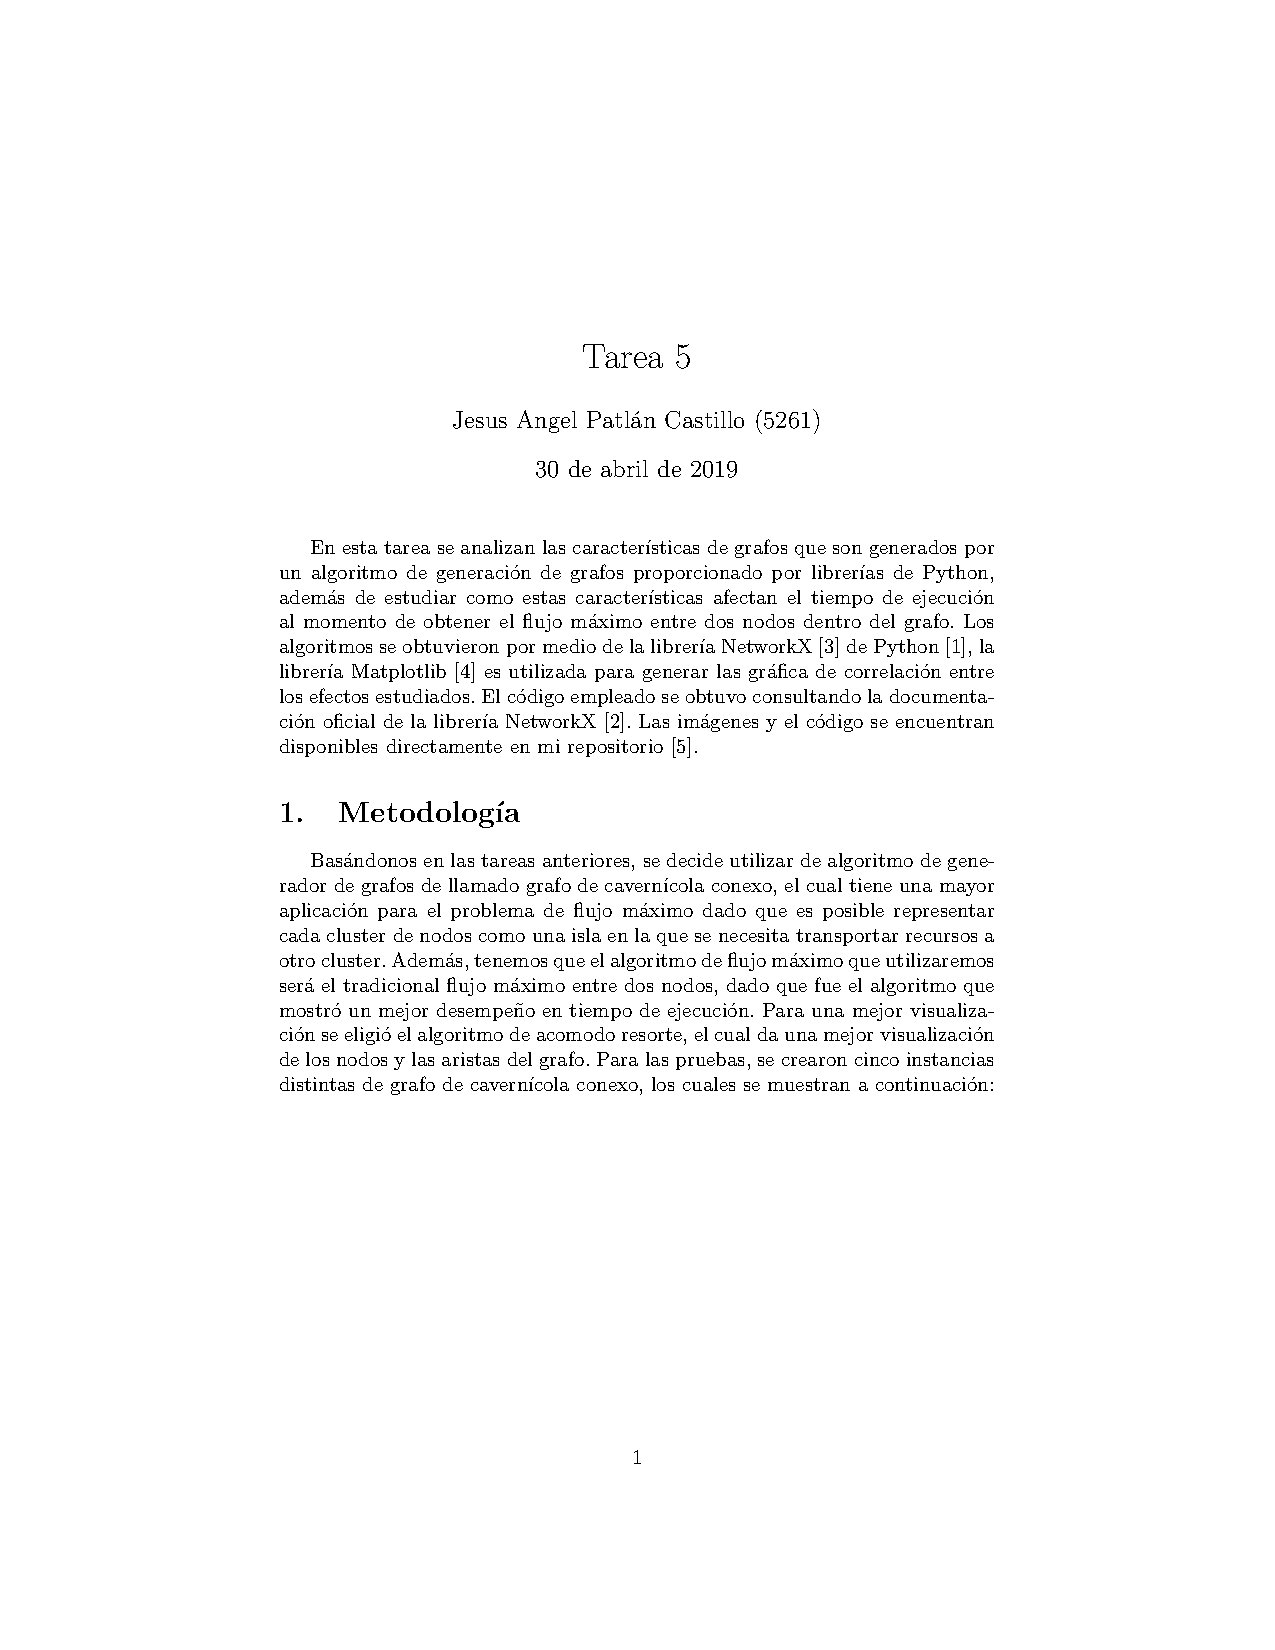
\includepdf[page=-]{5261-5-R}

\section{Conclusión de aprendizaje}
En este curso aprendí muchas propiedades acerca de los grafos y como estos impactan en el rendimiento de solución a problemas de flujo máximo, además de aplicar métodos estadísticos como ANOVA para determinar si ciertas propiedades del grafo tienen un impacto significativo directo en el tiempo de ejecución de los algoritmos utilizados en estas tareas.
Además, aprendí a utilizar el lenguaje Python para realizar las pruebas estadísticas y la generación de grafos, y dentro de Latex aprendí a utilizar diversos paquetes para el diseño de documentos y muchos aspectos claves para tener un trabajo limpio y formal. Me encuentro bastante satisfecho por lo aprendido en clase y considero que aprendí más de lo que esperaba, sobretodo sobre como elaborar un trabajo científico.

\bibliographystyle{plain}
\bibliography{references}

\end{document}
